\documentclass[10pt, a4paper, twocolumn]{article}
\usepackage[utf8]{inputenc}
\usepackage[T1]{fontenc}
\usepackage{graphicx}
\usepackage{beton}
\usepackage{eulervm}
\usepackage{amsmath}
\usepackage{bm}
\usepackage{microtype}
\usepackage[medium, compact]{titlesec}
%\usepackage[inline]{asymptote}
%\usepackage{tikz-cd}
\DeclareFontSeriesDefault[rm]{bf}{sbc}
% \usepackage{amssymb}
%% Turing grid is 21 columns (of 1cm if we are using A4)
%% Usually 4 "big columns", each of 4 text cols plus 1 gutter col;
%% plus an additional gutter on the left.
\usepackage[left=1cm, right=1cm]{geometry}
%\usepackage[Ragged, size=footnote, shape=up]{sidenotesplus}
\setlength{\columnsep}{1cm}
\title{Blockworld physics}
\author{}
\date{\today}

\begin{document}
\maketitle

\section{Earth blocks}

\subsection{General overview}

The challenge with Earth blocks is to model the hydrology: the
movement of water through the blocks.

Each Earth block contains some water. Water can move from block to
block. In real life, there are (I think!) two main processes: (1)
groundwater, which flows like a viscous fluid through saturated rock;
(2) moisture, which is transported via a diffusion-like process
(capilliary action, possibly?) in unsaturated rock.

Water tends to move:
\begin{itemize}
\item down, under gravity; 
\item from blocks with high pressure to blocks with low pressure; 
\item from blocks with high water content to blocks with low water
  content.
\end{itemize}

The following is a version of all of this. I am not claiming physical
realism with the real world but it is “physically plausible.”

\subsection{Block parameters}

All parameters are integers unless otherwise stated. An Earth block
has a single parameters, the water content, $w$.

The hydrostatic pressure, $p$, is then dervied from the water
content. See figure~\ref{fig:pressure} for the relationship between
the two.
\begin{figure}[ht]
  \centering
  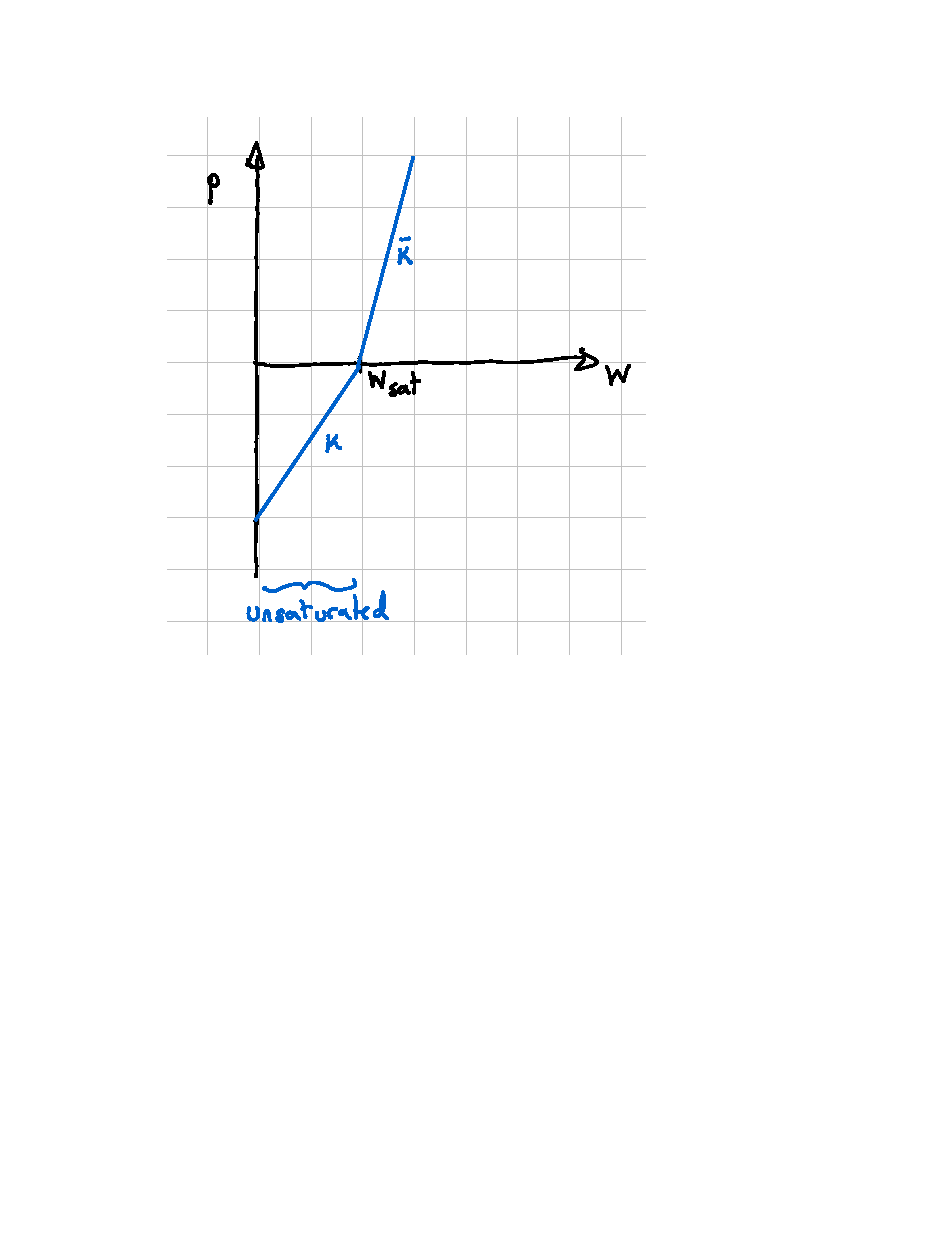
\includegraphics{fig-pressure.pdf}
  \caption{Dependence of hydraulic pressure on Earth block water
    content. Note that the pressure of an unsaturated block is
    effectively negative.}
  \label{fig:pressure}
\end{figure}

The units of pressure are length. A pressure of $1$ is the weight of
$1$ unit of water acting on an area of one block face. (Note that if
we had pure Water blocks, they would not necessarily be 1 unit of
water.)

\subsection{Global constants}

The following are the ``constants of nature.'' Their meaning is given
roughly here but the real meaning of these terms is just how they
enter into the equations of state.

\begin{enumerate}
\item Saturation level $w_{\text{sat}}$ (integer): the maximum water
  content per block.
\item Permeability: the inverse of the number of world ticks over
  which one unit of water flows between blocks subject to a pressure
  gradient of~$1$.
\item Gravitational constant is chosen to make the weight of 1 unit of
  water equal to~1.
\end{enumerate}
  
\subsection{Equations of motion}

This is a two-step algorithm. We start with the water content, $w$, of
each Earth block. The hydraulic pressure, $p$, of each block, is then
a piecewise linear function of~$w$, as described above.

\begin{enumerate}
\item Compute the water flux across each face.
  \begin{enumerate}
  \item For each face, compute the ``pressure gradient'' as the
    difference in $p$ between the two blocks separated by this
    face. In addition, if the face is a lower face, add a force that
    is the water content of the block above. (This is a gravitational
    term.)

  \item For each face, compute the \emph{preliminary flux} across that
    face is the pressure gradient times the permeability.

  \item Now potentially make adjustments to the fluxes. For each cell,
    consider all outgoing preliminary fluxes. We adjust these fluxes
    by ``giving $w$ to them in order from largest to smallest, until
    $w$ runs out,'' as follows. If the total outgoing preliminary flux
    is less that $w$, make no adjustment to the preliminary
    fluxes. Otherwise, start by assigning $w$ to the largest
    preliminary flux. If $w$ is less than the flux, adjust that flux
    to $w$ and the remaining fluxes to zero. Otherwise make no
    adjustment to the largest flux, subtract the largest flux from
    $w$, and continue with the next largest flux. Continue until there
    is no more water left.
  \end{enumerate}

\item For each cell, adjust its water content by the sum of the
  fluxes.
\end{enumerate}

\subsection{Boundary conditions}\label{sec:boundary}

Some Earth blocks abut other blocks. If the face is adjacent to Air,
treat it as an empty block with pressure zero. (At the moment, water
exiting into Air will be lost, but won't in fact happen very often.)

If the face is adjacent to Rock, treat the pressure gradient as zero
(so that there is no flux across this face).

\section{Light}

Light is a parameter of Air blocks. Light is $L_{\text{sky}}$ in any
block with unobstructed vertical line of sight to the sky; otherwise
it is $L_{\text{amb}}$. (Maybe we'll implement some radiosity model
later.)

\section{Plant}

A Plant block has two main components: the ``physical'' plant (which
follows ``physical laws'') and the controlling state machine. This
section describes the physical component.

The dynamic parameters of a Plant block are:
\begin{enumerate}
\item Water content (just like Earth blocks);
\item Energy content (another integer)
\end{enumerate}

The static parameters are:
\begin{enumerate}
\item Saturation level (as Earth blocks, but probably higher);
\item Compressibilities (saturated and unsaturated, like Earth
  blocks);
\item \ellipses
\end{enumerate}

\subsection{Plant actions}

Every state-machine tick, the Plant block can choose any number of the
following actions:

\begin{enumerate}
\item For each face, decide whether the water flow valve is open or
  closed. (That is, there is a choice of permeability.)
\item For each open face, a 
\end{enumerate}

\subsection{Plant sensors}

The plant state-machine has available to it the following data:
\begin{enumerate}
\item The face that is ``up.'' 
\end{enumerate}


\section{Wacky ideas section}

\begin{itemize}
\item When Plant blocks grow, they have to specify whether a face is a
  ``water in'' or ``water out'' face. 
\end{itemize}


\end{document}
